\section{Questionnaire}

\subsection{Création de questionnaires}
La problématique consistait à proposer un outil de création de questionnaire facile à
utiliser. Cet outil était un des besoins fondamentaux dans le projet qui nous a été 
donnés. La solution pour répondre au besoin formulé par le client que nous avons adopté, était de créer un générateur de questionnaires. L’utilisateur, à l'aide de celui-ci, peut créer des formulaires HTML en glissé-déposé. Étant donné que les utilisateurs de cet outil sont des non-informaticiens, on a adapté cet outil aux besoins de ces derniers pour le rendre plus facile aussi bien à l’utilisation qu'à la compréhension de son fonctionnement.

\begin{figure}[H]
    \begin{center}
	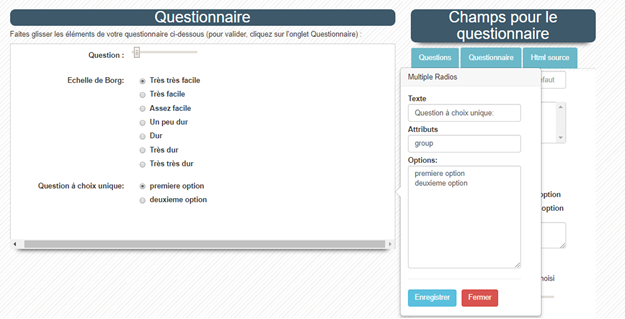
\includegraphics[scale=0.8]{img/questionnaire/modification}
    \end{center}
    \caption{Ajout d'une question dans le générateur de questionnaires}
\end{figure}


\subsection{Outil de création de questionnaire}
\subsubsection{Adaptation du besoin du client}


Cette interface permet à l'utilisateur de créer un questionnaire et paramétrer ses questions en glissant les questions de la partie droite vers la partie gauche et en cliquant sur la question déposée, un nouveau formulaire apparaît avec un nombre de zones de texte différent selon le type de question. Ce formulaire permet de modifier ou remodifier la question.


\begin{figure}[H]
    \begin{center}
	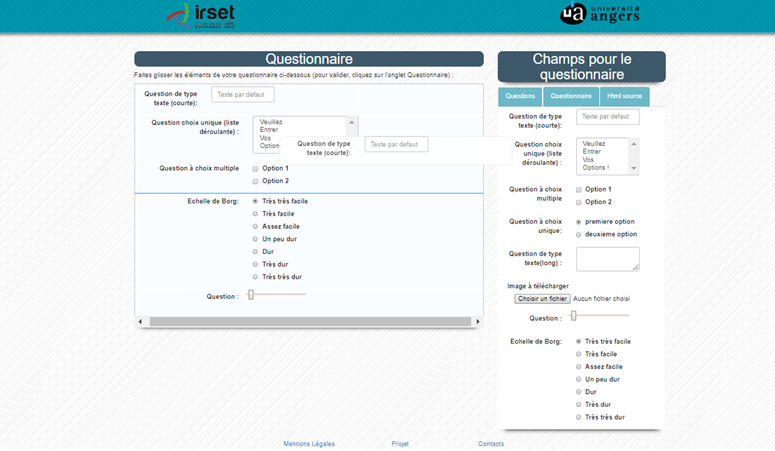
\includegraphics[scale=0.8]{img/questionnaire/generateur}
    \end{center}
    \caption{Modification d'une question}
\end{figure}
 
 
\subsubsection{La gestion des questions}

Pour supprimer une question, il suffit de glisser la question hors du cadre. Cela permet de la retirer des autres questions.


\begin{figure}[H]
    \begin{center}
	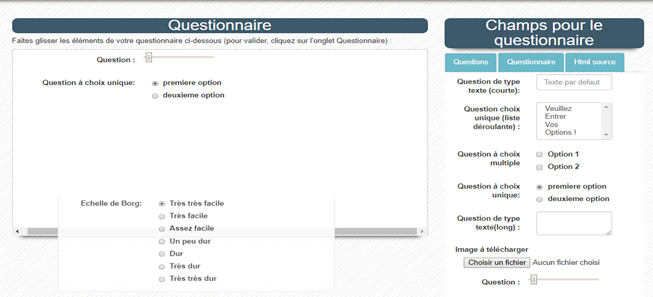
\includegraphics[scale=0.8]{img/questionnaire/suppresion}
    \end{center}
    \caption{Suppression d'une question}
\end{figure}


\subsubsection{Réorganisation des questions}

Lorsqu'on souhaite repositionner les questions, nous avons fait en sorte qu'il suffise de glisser puis déposer les questions à l'endroit où nous souhaitons la placer (en restant dans le même cadre).



\begin{figure}[H]
    \begin{center}
	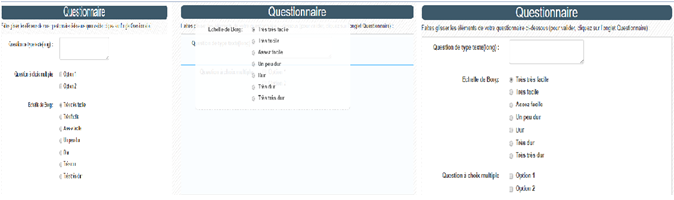
\includegraphics[scale=0.8]{img/questionnaire/repositionnement}
    \end{center}
    \caption{Repositionnement des questions}
\end{figure}

\subsubsection{Sauvegarde du questionnaire}

Pour finaliser la création d’un questionnaire, il faut que l’utilisateur saisisse le nom et l’identifiant du questionnaire puis en cliquant sur le bouton enregistrer. Le questionnaire va être sauvegardé en deux formes différentes, la première est sous forme d’un fichier HTML (figure 3.9) et la deuxième est dans la base de données qu’on peut consulter à partir de la liste des questionnaires (figure 3.10).


\begin{figure}[H]
    \begin{center}
	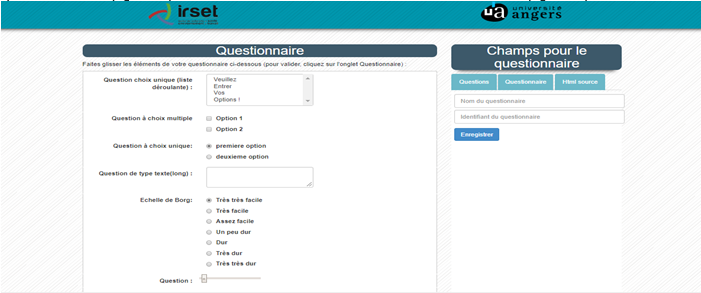
\includegraphics[scale=0.7]{img/questionnaire/enregistrement}
    \end{center}
    \caption{Saisire de données pour finaliser la sauvegarde}
\end{figure}


\begin{figure}[H]
    \begin{center}
	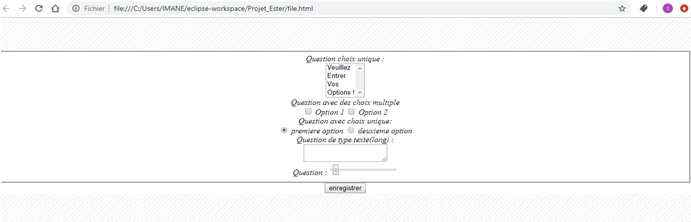
\includegraphics[scale=0.7]{img/questionnaire/fichier}
    \end{center}
    \caption{Sauvegarde sous forme d'un formulaire HTML}
\end{figure}

\begin{figure}[H]
    \begin{center}
	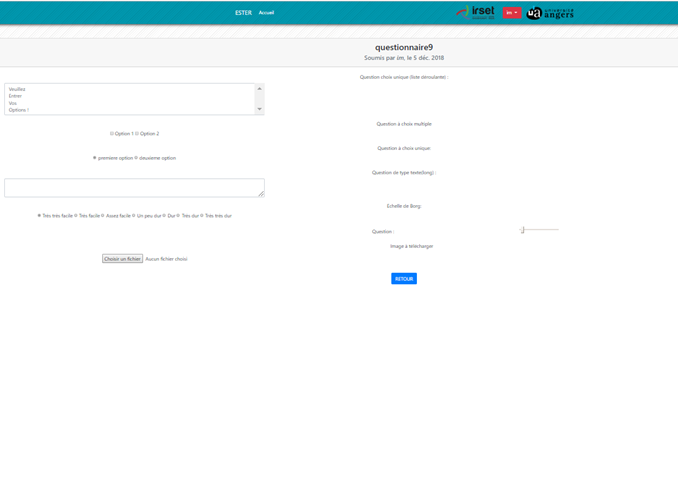
\includegraphics[scale=0.7]{img/questionnaire/affichage}
    \end{center}
    \caption{Affichage du questionnaire enregistré dans la base de données}
\end{figure}